\review{The authors have addressed many of my previous comments. However, there are still several major issues that need further clarification.}

\vspace{1eM}
\underline{\textit{Reply:}} We thank the reviewer for providing further useful comments which help us to greatly improve the manuscript.

\begin{enumerate}
	
	\cmnt{1} \review{The revised paper did not address my previous comment about how to select the sub-channel ordering. I understand that finding the best sub-channel ordering requires exhaustive search which has extremely high complexity. But it is important to provide a guidance on what would be a good choice of sub-channel ordering. For example, can we achieve a good performance by using a low complexity ordering algorithm such as a greedy sub-channel ordering algorithm?}
	
	\resp We apologize for not clarifying the sub-channel ordering in detail in our previous manuscript. For simplicity we use random sub-channel ordering in our paper. That is, after finding the precoders for a current sub-channel, we can choose any previously unselected sub-channels as the next candidate sub-channel for which the precoders are identified using the updated backlogged packets. As suggested by the reviewer, the greedy sub-channel ordering can also be considered while selecting the order. The greedy ordering can be based on sorting the best channel gain from each sub-channel, which is obtained by finding the highest channel norm seen between any user and the corresponding serving \ac{BS}.  
	
	We remark that the choice of a sub-channel ordering scheme should also consider the number of backlogged packets associated with each user. We have emphasized this issue by comparing various ordering schemes for the same system model with two different set of backlogged packets associated with each user. We do not include in the manuscript due to space limitations, we have included in the response letter to answer the reviewers' question. We considered a system with \eqn{N = 4} sub-channels, \eqn{N_B = 2} \acp{BS} with \eqn{N_T = 4} transmit antennas and \eqn{K = 12} single antenna users. The \ac{PL} is distributed uniformly over \eqn{[0,-3]} dB. The number of backlogged packets assumed for each user is provided in the corresponding captions in Figure \ref{fig-review-1}.
	\begin{figure*}[h!]
		\centering
		\subfloat[][Number of backlogged packets for each user in bits \eqn{Q_k = [11,8,14,6,6,2,10,10,5,6,9,5]}]{
			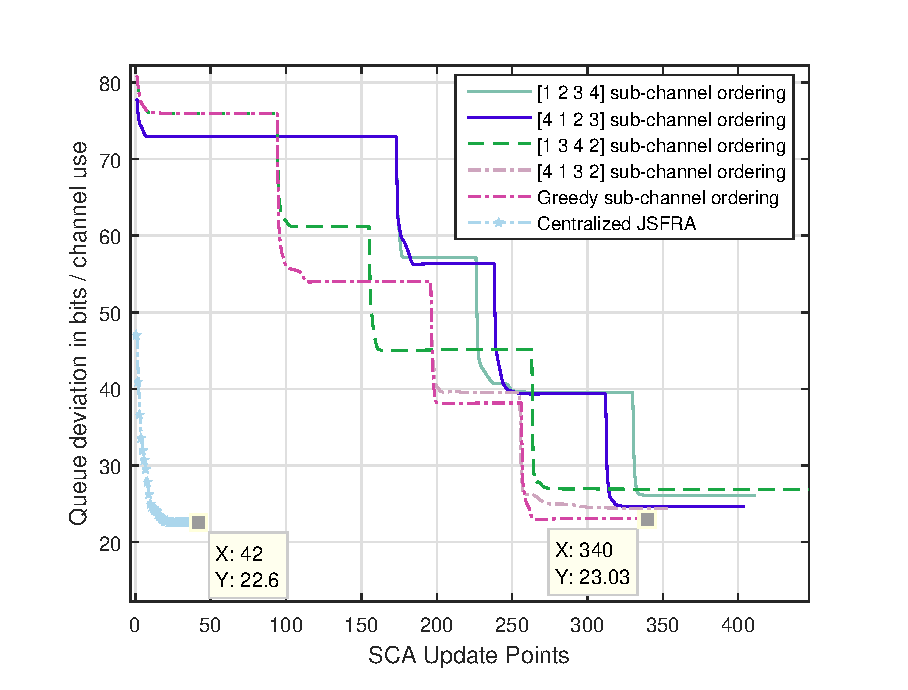
\includegraphics[width=0.8\textwidth]{reviewer_2_Q1B.eps}
			\label{fig-review-1a}
		}
		\hfill
		\subfloat[][Number of backlogged packets for each user in bits \eqn{Q_k = [8,9,12,8,12,5,4,10,8,5,7,9]}]{
			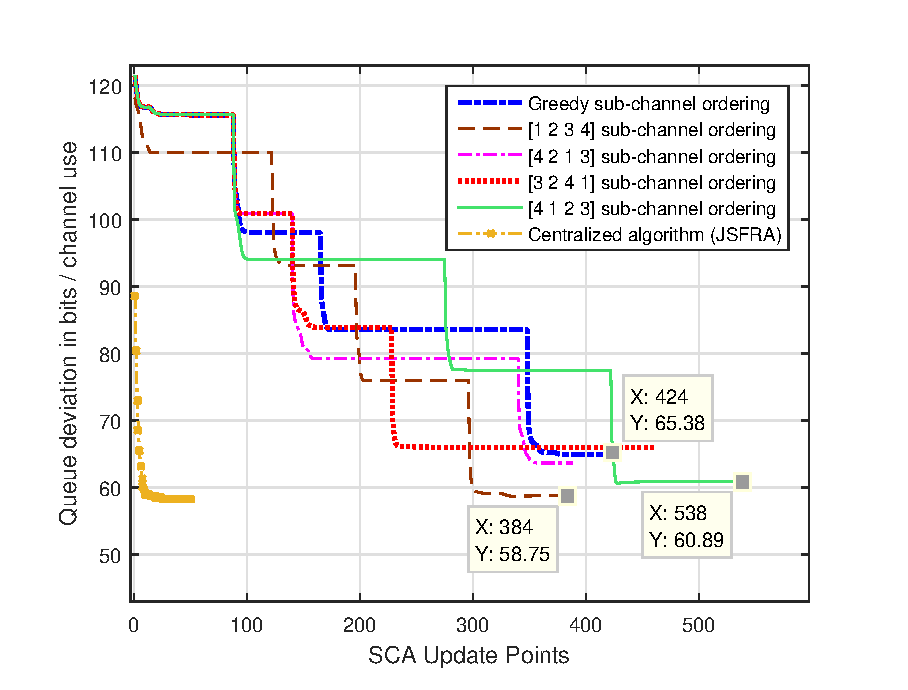
\includegraphics[width=0.8\textwidth]{reviewer_2_Q1A.eps}
			\label{fig-review-1b}
		}
		\caption{Convergence of the algorithms for \me{\lbrace N,N_B,K,N_T,N_R \rbrace = \lbrace 4,2,12,4,1 \rbrace} using \me{\ell_1} norm}
		\label{fig-review-1}
	\end{figure*}
	
	Figure \ref{fig-review-1} compares different sub-channel ordering schemes in terms of the total number of backlogged packets remaining in the system. As can be seen from Figure \ref{fig-review-1}\subref{fig-review-1a}, the greedy sub-channel ordering provides a favorable way of choosing sub-channels to minimize the total number of backlogged packets. However in Figure \ref{fig-review-1}\subref{fig-review-1b}, it is evident that the greedy sub-channel ordering is no longer better in comparison to the few other random ordering schemes. We have included the discussions regarding the greedy sub-channel ordering in the revised manuscript as a heuristic method under Section III-D final paragraph. However, as the number of users in the system increases, all sub-channel ordering schemes are similar in minimizing the total number of backlogged packets in the system without any noticeable gain.
	
	\cmnt{2} \review{The authors mentioned that the signaling overhead of the distributed algorithm can be reduced by using a smaller number of iterations \eqn{J_{\max}}. But still, you didn't answer my question about whether the signaling overhead of the distributed algorithm is smaller than the centralized algorithm. You should first analyze the signaling overhead of the distributed algorithm for fixed \eqn{J_{\max}} and the signaling overhead of the centralized algorithm. Then you should point out under what \eqn{J_{\max}} the distributed algorithm will have less signaling overhead than the centralized algorithm. Is it possible that the distributed algorithm always has more signaling overhead than the centralized algorithm even when \eqn{J_{\max} = 1}? Finally, there is a trade-off between performance and signaling overhead (\eqn{J_{\max}}) for the distributed algorithm. For the same signaling overhead (we can control \eqn{J_{\max}} to make the signaling overhead of the distributed algorithm approximately equal to that of the centralized algorithm), does the distributed algorithm achieve better performance than the centralized algorithm?}
	
	\resp
	We thank the reviewer for the insightful comment and we apologize for the lack of clarity in explaining this information in our earlier manuscript.
	\begin{enumerate}
		\item The amount of signaling overhead of the distributed algorithm and the centralized one depends on the system model of consideration. For example, let us consider a model with \eqn{N = 1} sub-channel, \eqn{K = 4} users and \eqn{N_B = 2} \acp{BS}, each serving 2 users. Let \eqn{N_T = 4} be the number of transmit antennas and \eqn{N_R = 1} be the number of receive antennas at each user. We note that a centralized algorithm requires the knowledge of all channels matrices in the system and thus the resulting amount of information exchange is proportional to the product of the numbers of users (\eqn{K}), \acp{BS} (\eqn{N_B}), and transmit and receive antennas (\textit{i.e.}, \eqn{N_T} and \eqn{N_R}).
		
		In order to quantify the total number of bits required in a centralized solution, let us assume that each complex channel for a \ac{SISO} model requires \eqn{10} bits, \textit{i.e}, \eqn{4} bits for amplitude and \eqn{6} bits for phase (assuming phase is more important) or it can be a equal share of \eqn{5} bits for both amplitude and phase. Using this assumption, the total number of bits for channel information to be exchanged via backhaul is \eqn{10 \times K \times N_B \times N_R \times N_T = 320} bits. On the other hand, for the distributed algorithms, let us consider \eqn{6} bits for quantizing each element of the consensus vectors. Consequently, the proposed distributed solutions require \eqn{6 \times 2 \times 2} bits to be exchanged in each iteration. 
		
		In the above example, for the same signaling overhead as in centralized method, we can perform only up to 6 \ac{SCA} updates for \eqn{J_{\max} = 2} (\textit{i.e.}, two updates for \ac{ADMM} part). This may not be sufficient for the distributed algorithms to attain the same performance as the centralized method. However, as the number of sub-channels, users and/or the antenna elements increases, it may not be a feasible option to send complete \acp{CSI} across the coordinating \acp{BS} to the centralized controller in the current cellular systems. In addition to comparing the signaling overhead, we also need to consider the performance loss due to the \ac{CSI} quantization in the centralized approaches, which is beyond the scope of our paper. Generally, the performance is significantly degraded if precoders are designed with the quantized \ac{CSI} as discussed in [R1]. Moreover, in the centralized algorithm, resulting transmit precoders need to be exchanged with the corresponding \acp{BS} before the actual transmission, which involves significant overhead in the backhaul usage.
		
		\vspace{1eM}
		[R1] Muhammad-Fainan Hanif, Le-Nam Tran, Antti Tölli, Markku Juntti,  and Savo Glisic, "{Efficient Solutions for Weighted Sum Rate Maximization in Multicellular Networks With Channel Uncertainties}'', \textit{IEEE Trans. Signal Process}., vol 61, no. 22, pp. 5659-5674, Nov. 2013.
		\vspace{1eM}
		
		\item Using the above discussion, we can say that when the system size is huge, it would be favorable to consider the distributed algorithm over the centralized approach due to the huge signaling overhead involved in exchanging the channels.
		
		\item From the above discussions, we can see that the \ac{ADMM} and primal schemes require significant overhead compared to the centralized algorithms for a small system. However, for a system involving more coordinating \acp{BS}, users and antenna elements, it would be beneficial to use the proposed distributed algorithms with \eqn{J_{\max} > 1} to have a strictly monotonic decrease in the objective. If we set \eqn{J_{\max} = 1}, the convergence of the proposed algorithms is not guaranteed as shown in Figure \ref{fig-review-2-a}. The system model considered is the same as the one used for Figure \ref{fig-review-1}\subref{fig-review-1a}.
		\begin{figure}[h!]
			\centering
			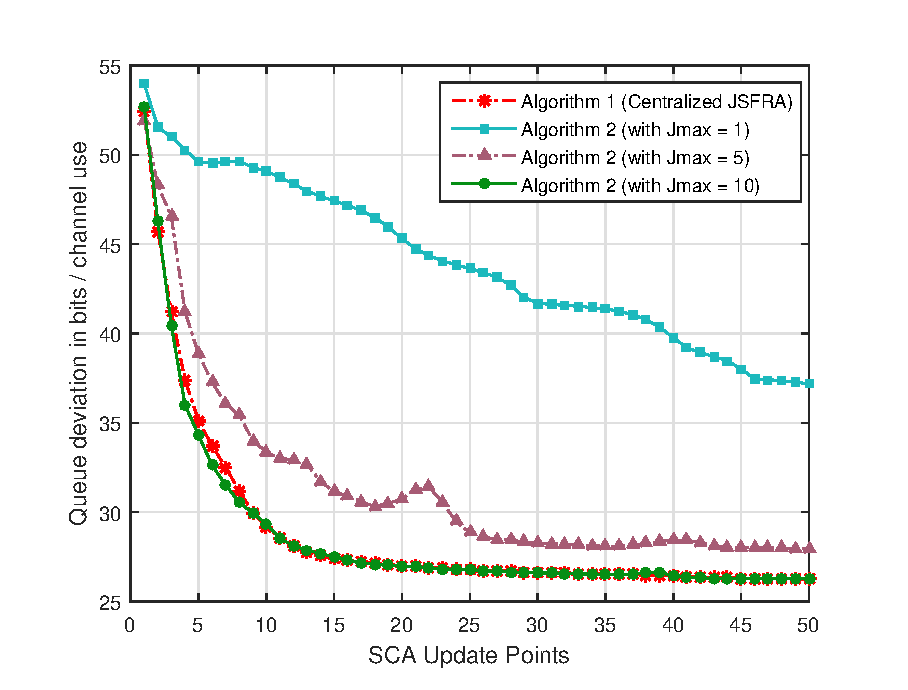
\includegraphics[width=0.8\columnwidth]{reviewer_2_Q1C.eps}
			\caption{Convergence of the centralized and distributed algorithms for \me{\lbrace N,N_B,K,N_T,N_R \rbrace = \lbrace 4,2,12,4,1 \rbrace} using \me{\ell_1} norm}
			\label{fig-review-2-a}
		\end{figure}
		Note that Figure \ref{fig-review-2-a} plots the queue deviation at the \ac{SCA} update points only. The number of backlogged packets in each \ac{ADMM} iteration is not shown for clarity reason.		
		
	\end{enumerate}
	
	The above discussion is included in a condensed form in the first and the last paragraph of Section IV-C. 
	
	In reality, since the channel is time-correlated, it is enough to update the precoders once per radio frame. Thus, it is not necessary for the distributed algorithm to converge until the end. Instead, the decentralized parts only need to follow the fading process when \eqn{J_{\max} > 1}. The performance of the distributed algorithm based on the dual decomposition scheme was discussed for the time-correlated fading in Section C of [12], which showed that it is enough for the distributed precoder design to follow the fading process to provide the desired performance. Studying the performance of distributed algorithms for the time correlated case is beyond the scope of our paper and thus is not considered in the current manuscript. However, we take this opportunity to show a plot demonstrating this behavior for the \ac{KKT} based algorithm presented in Section IV-C of the manuscript.
	\begin{figure}[h!]
		\centering
		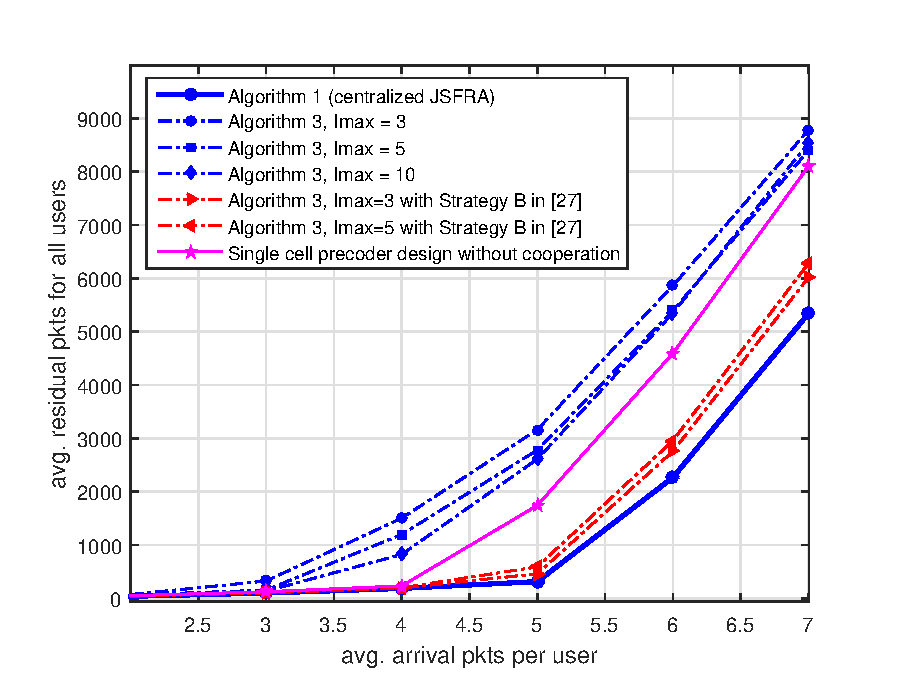
\includegraphics[width=0.8\columnwidth]{reviewer_2_Q2.eps}
		\caption{Expected number backlogged packets after each transmission instant for a system \me{\lbrace N,N_B,K,N_T,N_R \rbrace = \lbrace 4,2,16,4,2 \rbrace} evaluated for \eqn{500} slots}
		\label{fig-review-2}
	\end{figure}
	
	Figure \ref{fig-review-2} compares the performance of the distributed \ac{KKT} approach, \textit{i.e.}, Algorithm 3 for different values of \eqn{I_{\max}}. The signaling requirements are outlined in Algorithm 3 and the overhead involved in the signaling is penalized in the achievable rate of the users.\footnote{Please refer to [27] for further details.} We considered that the channel is coherent over \eqn{N_S = 100} symbols and the precoder update is performed by exchanging the required information for \eqn{J_{\max} = 3,5,10}. The overhead is considered as \eqn{\tilde{t}_{l,k,n} = (1 - \frac{J_{\max}}{N_S}) \times t_{l,k,n}}, where \eqn{\tilde{t}_{l,k,n}} is the rate seen by the user and the factor \eqn{(1 - \frac{J_{\max}}{N_S})} is considered as a penalty involved due to the precoder exchange as discussed in [R2] and [R3]. The average number of backlogged packets after each transmission slot is evaluated as 
	\begin{equation}
	\chi = \sum_{k = 1}^K \; [ Q_k - \tilde{t}_k ]^+
	\end{equation}
	
	Unlike Algorithm 3, the centralized scheme presented in Figure \ref{fig-review-2} has no penalty term and it is used as a benchmark. In order to improve the performance of the distributed scheme, the operating point involved in the \ac{SCA} algorithm is considered from the earlier frame instead of begin generated randomly. 
	
	\begin{comment}
	Since we use \ac{KKT} approach, we can either use all users in the system for the precoder design or we can utilize single-cell MU-MIMO user selection presented in the literature to limit the number of users for which the precoders are designed, which leads to the faster convergence. As we can see from Figure \ref{fig-review-2}, as the arrival rate per user increases, the performance of \ac{KKT} schemes with \eqn{J_{\max} = 3,5,10} converges since the number of backlogged packets are significantly large, therefore, the same set of users will be served by the algorithm with better precoders by utilizing the memory. 
	
	In spite of using memory and prior scheduling in the \ac{KKT} approach, isolated single \ac{BS} processing performs much better than the distributed scheme due to the limited number of iterations allowed in the algorithm. Note that the precoders are not updated for the desired users until convergence, after the limited number of iterations. However, if we perform the single cell precoder design by considering the neighboring precoders as fixed after the recent exchange as discussed in [28], we can improve the performance significantly for Algorithm 3 as shown by red curves in Figure \ref{fig-review-2}. In this approach, in between each exchange across the coordinating \acp{BS}, each \ac{BS} will perform \eqn{J_{\max} = 20} with the neighboring precoders as fixed. Once the iterations are performed to update the precoders, it is then exchanged across the coordinating \acp{BS} to perform the same procedure as mentioned earlier. 
	\end{comment}
	
	\vspace{1eM}
	[R2] Changxin Shi, Berry R.A., Honig M.L., ``{Bi-Directional Training for Adaptive Beamforming and Power Control in Interference Networks}," \textit{IEEE Transactions on Signal Processing}, vol.62, no.3, pp.607,618, Feb.1, 2014
	
	[R3] P. Jayasinghe, A. T\"{o}lli, J. Kaleva,  M. Latva-aho, "{Bi-directional Signaling for Dynamic TDD with Decentralized Beamforming}'', in \textit{Proceedings of IEEE ICC SmallNets Workshop}, London, UK, June, 2015		
	\vspace{1eM}
			
\cmnt{3} \review{If the authors can't prove the convergence of the ADMM algorithm (or the decomposition approach via KKT conditions) in Section IV.B, then at least, you should discuss the property of the fixed point of the algorithm. For example, does there exist a fixed point of the algorithm? If so, is the fixed point of the algorithm unique? Is any fixed point of the algorithm also the optimal solution of the original problem in (20)? Assuming that the ADMM algorithm converges to a fixed point, will the interference vector in (39) converges to the actual interference in the network? These questions must be clarified in the paper. Otherwise, it is not clear how the ADMM algorithm is related to the original problem in (20). Similar questions should also be answered for the decomposition approach via KKT conditions. }

\resp We thank the reviewer for raising the important concern regarding the convergence issue of the distributed algorithms. We want to clarify that we are able to prove the convergence of Algorithm 2 which is based on \ac{ADMM}. In our paper the number of updates for the \ac{ADMM} part is denoted by \eqn{J_{\max}}. There is a trade-off between signaling overhead and achievable performance by varying \eqn{J_{\max}}. In reality we may set \eqn{J_{\max}} to a finite value to reduce the signaling overhead. In such a case, the convergence is not guaranteed. In our simulations, the \ac{ADMM} part can find an optimal solution to the (convex) subproblem in each \ac{SCA} step when \eqn{J_{\max} = 20}.

\begin{itemize}
\item The fixed point for the algorithm exists if the distributed approaches are performed until convergence or iterated for significant number of iterations to ensure strict monotonicity of the objective in each \ac{SCA} step. In such scenarios, the iterative method in Algorithm 2 finds a fixed point such that \eqn{\mc{A}(\mbf{x}^{\ast}) = \mbf{x^{\ast}}}, \eqn{\forall \mbf{x}^{\ast} \in \mc{F}^{\ast}}, where \eqn{\mc{F}^{\ast}} is the set of all fixed points of the algorithm and \eqn{\mc{A}} denotes the Algorithm 2 at each \ac{AO} update point as in (54).

\item Note that in each \ac{SCA} step, the iterative procedure in Algorithm 2 finds a (unique) solution by solving (20) or (28) with the previous solution as the operating point. Therefore, the fixed point of Algorithm 2 depends on the initial operating point chosen for the iterative procedure. Upon convergence, the fixed point of Algorithm 2 can be distinct for different starting points chosen to initialize the iterative procedure.

\item Since the original problem is nonconvex, there exists multiple stationary point. Therefore, if the Algorithm 2 is initialized with a feasible operating point, then the limit point of the iterative algorithm is a fixed point of Algorithm 2, provided strict monotonicity of the objective and the uniqueness of the iterates are ensured in each \ac{SCA} step. Due to the fact that the limit point depends on the chosen initial operating point, there exists a set of limit points, which are also a fixed point of Algorithm 2. Therefore, all fixed points found by Algorithm 2, satisfying strict monotonicity and the uniqueness of the iterates in each \ac{SCA} step, are stationary points of the original nonconvex problem (16).

\item We also want to remark that  the proposed distributed algorithms are not based on fixed-point theory. The \ac{ADMM} part is to find a (unique) optimal solution to the strongly convex subproblem in each \ac{SCA} step. More explicitly, the \ac{ADMM} approach is used to solve the problem given in (20) based on augmented Lagrangian function which is different from fixed-point theory. However, the optimal solution of (20) is not necessarily a fixed-point of the problem. 

\item When the ADMM approach converges, the interference vector is guaranteed to be equal to the actual interference seen in the network. This is the main principle of \ac{ADMM} where the local variables (the vectors in (38)) converge to the global variables (the actual inference vectors).

\item Another point we want to make is that Algorithm 2 yields a stationary point of the original noncovex problem upon convergence and this stationary point may not be a fixed-point of the original noncovex problem, \textit{i.e.}, \eqn{f(\mbf{x}) = \mbf{x}}. 

\item Since Algorithm 3 is based on a heuristic iterative approach to find a solution of \ac{KKT} equations, we cannot prove its convergence. When Algorithm 3 terminates, we will use the transmit and receive beamforming vectors to calculate the original objective.

\end{itemize}

We have updated the manuscript to clarify all the points mentioned above. Please refer to Section IV-B last paragraph after (40) in the revised manuscript. Additional information regarding the convergence of the distributed algorithms is provided in Appendix B second paragraph. The discussion on the convergence of the KKT based approach for MSE reformulation scheme is also presented in Appendix B last paragraph. For reference purpose, we have also referred the interested reader to [10], which discusses exclusively about the ADMM approach.

\begin{comment}
\resp We thank the reviewer for raising the concern regarding the convergence of the distributed algorithms with limited number of iterations. In view of this, we have updated the manuscript to include discussions on the convergence of the distributed algorithms with a limited number of iterations in the third paragraph of Appendix B after (57). Since the monotonicity of the algorithm with limited number of updates in each subproblem is not guaranteed in each iteration, it is hard to prove the convergence of the overall algorithm. However, if the algorithm is allowed to converge or iterated enough to guarantee the strict monotonicity of the objective in between the \ac{SCA} updates, the global convergence of the algorithm to a limit point of the original nonconvex problem is guaranteed based on the discussions provided in Appendix A.
\begin{itemize}
\item If there exists a fixed point or a set of fixed points for the original nonconvex problem in (16), then the proposed centralized algorithm in Section III-B and III-C finds at least one such point if iterated until convergence, which is provided in Appendix A. In order to find a unique fixed point, we regularize the objective function in (16) with a quadratic penalty term as discussed in Appendix A to transform the objective as a strongly convex function.
\item If the distributed algorithm is carried out for a limited number of iterations, it is not guaranteed to achieve a fixed point even if the outer \ac{SCA} update is performed for a large number of iterations. By this approach, the distributed approaches are not guaranteed to converge to a stationary point. In all our simulations on the primal and the \ac{ADMM} approach, we have set \eqn{J_{\max} = 20} in order to guarantee the monotonicity of the objective.
\item Unless the objective function is regularized with a strongly convex term as in Appendix A-C, the uniqueness of the iterates is not guaranteed. 
\item In each \ac{SCA} update, if the distributed algorithms are allowed to converge to the centralized solution, then the overall convergence will be a stationary point of the original nonconvex problem by following the same argument as that of the centralized algorithm.
\item Since the coupling between the distributed precoder designs is the interference between the BSs and the users, in the \ac{ADMM} approach, the interference is treated as a local variable, which is then included in the precoder design problem for each coordinating BS. This is treated as a local variable for individual \acp{BS}. Note that the local variable is an assumption made by the BS on the actual interference caused by the neighboring BSs. Since the actual interference caused is different, the consensus has to be made between the local interference variable maintained at each BS with the global consensus interference variable, which is nothing but the average between the corresponding BSs interference. These discussions have been made in the revised manuscript in Section IV-B. For reference purpose, we have also referred the interested reader to [11], which discusses exclusively about the ADMM approach. Upon convergence of the \ac{ADMM} approach, the interference vector is equal to the actual interference seen in the network.
\end{itemize}

\end{comment}

\end{enumerate}
